\chapter{What tail recalibration improves}
\label{ch:tailresults}

The opportunity for residual correction depends on the original tail forecast. We first test correction against simulated truth, then evaluate it on 28 equity indices. These comparisons show the clearest market benefit for Gaussian tails, while leaving additional neural improvement in the joint score uncertain.

The neural comparisons convert an archived variance path to Student-$t_8$ tails; they use neither the native mixture nor the corrected five-model set. Specialist tables retain their historical fitting policy, with convergence-checked replay reported separately in Appendix~\ref{sec:optimizer-sensitivity}. Prior contact with every market panel remains documented in Section~\ref{sec:exposure}.

\section{Why these comparisons?}

We compare forecasts with different possible errors: Gaussian and Student EWMA, historical simulation, Student GARCH, Gaussian tails on the same GARCH scale, GAS VaR--ES and archived neural variance. FHS supplies the established residual alternative \citep{baroneadesi1999var,baroneadesi2008garch}. Holding GARCH scale fixed across its two tail laws helps distinguish tail-conversion repair from improved volatility prediction.

FZ0 is the main score for the VaR--ES pair at 5\%, 2.5\% and 1\%; breach frequencies and ES residuals are secondary diagnostics. Development covers 2011--2014 and the later panel 2015--February 2022. Paired comparisons give markets equal weight and use synchronised calendar-block intervals. Under the historical protocol, these are marginal intervals rather than joint coverage of all comparisons.

The later evaluation retains the development-selected 1,000-residual guard, even if a different choice appears better afterwards. Appendix~\ref{sec:tail-score-details} records decisions, tolerances and the post-hoc Holm adjustment. Convergence-checked replay on the same observations preserves the principal decisions.

\section{Controlled experiments: correction error and potential benefit}

Simulation provides a reference unavailable in markets: the generating process's true conditional VaR and ES, termed the \emph{oracle}. Correcting this pair tests estimation damage, while correcting a Gaussian forecast tests repair of unsuitable shape. We use stable Student-$t_5$ GARCH, stable Student-$t_5$ switching volatility, and GARCH whose innovations switch halfway from Student-$t_8$ to Student-$t_3$. The 1,620 forecaster, tail, length and seed combinations cover three tail levels, six lengths from 1,000 to 32,000 and five seeds. Scoring starts after 250 observations.

\begin{figure}[!htbp]
\centering
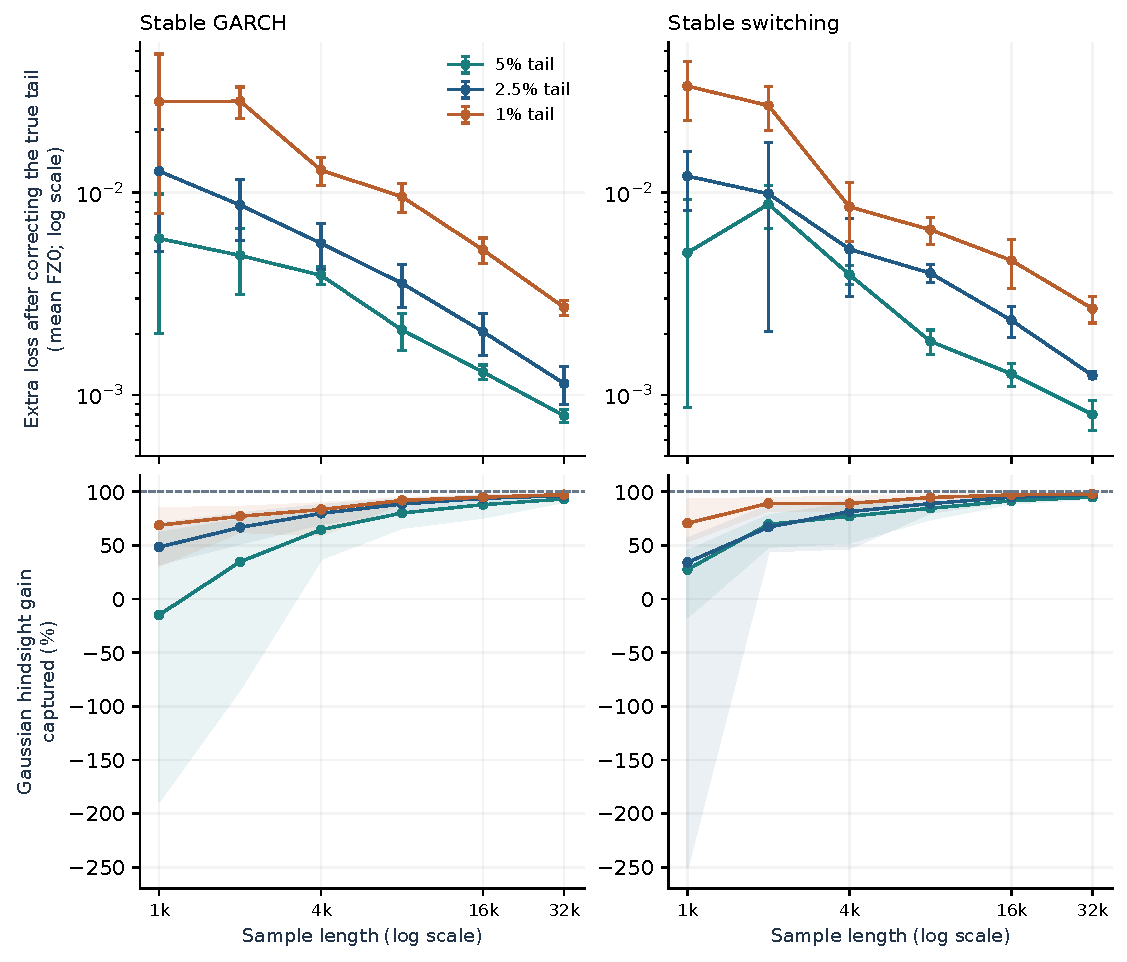
\includegraphics[width=\textwidth]{tail_learning_curves.pdf}
\caption[Tail-correction error and recovered benefit across sample sizes]{Stable Student-$t_5$ simulations at all six scheduled lengths. Top: mean FZ0 increase after correcting the known true tail forecast, with one standard error across five seeds. Bottom: ratio of mean Gaussian-forecast improvement to mean constant-ratio hindsight improvement; shading spans the five individual ratios and the horizontal line marks $100\%$. The hindsight fit uses scored outcomes. These descriptive curves and seed ranges are not confidence bands or general performance guarantees.}
\label{fig:tail-learning}
\end{figure}

As residual history grows, the error introduced by correcting the true forecast generally declines (Figure~\ref{fig:tail-learning}). On long stable paths, Gaussian correction recovers about 93--98\% of the hindsight improvement. The two comparisons show the benefit of repairing Gaussian tails and the estimation cost of correcting the true pair. The recovery ratio divides sample mean gains by a gain from fitting scored outcomes. Small denominators can make the ratio unstable, and realised harm can make it negative. Five seeds describe simulation variation without establishing a universal rate or a market-window choice.

\subsection{Changing tails and the limits of full history}

The halfway law change tests the limitation of full history. Correcting the true pair produces excess losses near 0.005 and 0.007 at 5\% and 2.5\%, exceeding historical tolerance. Pre-change residuals remain in the estimate, so the fitted tail mixes both laws and adapts slowly. Gaussian correction still improves the score over the complete path. This controlled result neither selects an optimal window nor shows that the guard detects a change in time.

\subsection{Retaining the daily scale}

\begin{figure}[!htbp]
\centering
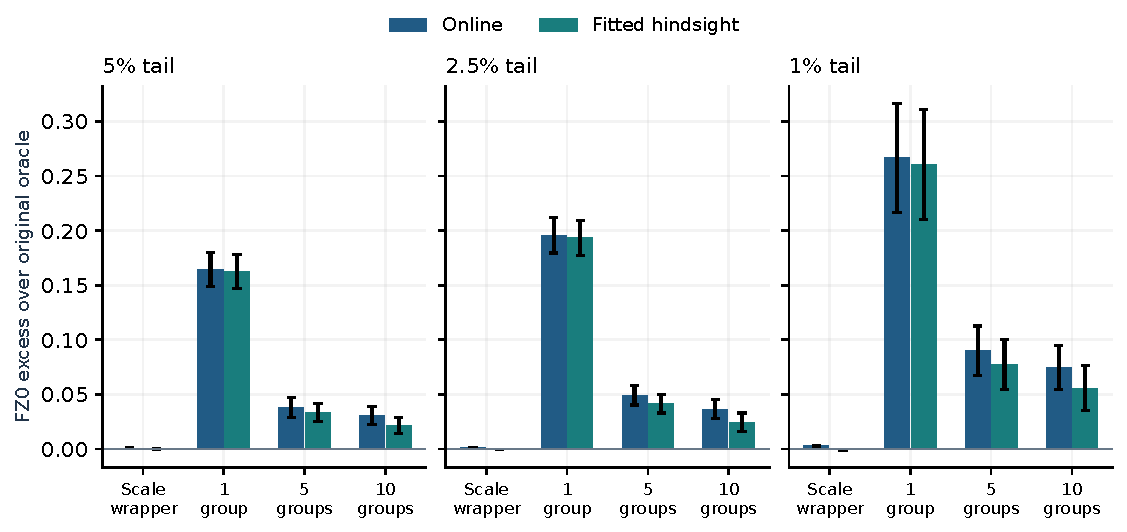
\includegraphics[width=\textwidth]{tail_grouping_cost.pdf}
\caption[What grouping loses when the daily scale is informative]{Stable GARCH oracle at $T=32{,}000$, with five simulation seeds. Bars show mean FZ0 excess over the original oracle; error bars are one standard error across seeds. Online estimates and hindsight fits on the scored sample are separate objects. One, five and ten groups replace the varying scale by constant raw-return pairs within groups; the scale wrapper retains daily scale. Fitted-hindsight excess is not the population approximation floor.}
\label{fig:tail-grouping}
\end{figure}

Grouping replaces each day's changing tail pair with a constant pair within its group. More groups preserve finer scale detail but provide fewer tail observations per estimate (Figure~\ref{fig:tail-grouping}). Online results favour retaining scale in stable GARCH. Hindsight fits see scored outcomes and can fit noise, so their differences measure neither irreducible error nor achievable online gain. The finding concerns these procedures rather than all grouped calibration methods.

\section{Gaussian forecasts: the clearest improvement}

The Gaussian comparison asks whether the guard improves on each original tail pair on the same market observations. Gains are original minus guarded FZ0, so positive values favour correction. Each panel combines two base models and three tail levels.

\begin{table}[htbp]
\centering
\caption[Historical Gaussian-tail improvements and multiplicity]{Historical fixed-guard Gaussian comparisons. Gains are original minus guarded FZ0; positive is favourable. Holm-adjusted $p$-values adjust the six Gaussian-tail comparisons within each panel, post hoc. GARCH rows retain the original optimiser acceptance policy; the convergence-checked sensitivity is separate.}
\label{tab:tail-m1}
\small
\begin{tabular}{llrrrrr}
\toprule
Panel & Base model & $\alpha$ & Gain & Improved & Raw $p$ & Holm $p$\\
\midrule
Development & EWMA Gaussian & .050 & .0266 & 26/28 & .025 & .100\\
 & GARCH Gaussian & .050 & .0045 & 21/28 & .365 & .365\\
 & EWMA Gaussian & .025 & .0659 & 27/28 & .004 & .020\\
 & GARCH Gaussian & .025 & .0173 & 19/28 & .127 & .254\\
 & EWMA Gaussian & .010 & .1613 & 25/28 & .001 & .006\\
 & GARCH Gaussian & .010 & .0534 & 20/28 & .049 & .147\\
\midrule
Later & EWMA Gaussian & .050 & .0297 & 26/28 & .004 & .012\\
 & GARCH Gaussian & .050 & .0035 & 17/28 & .136 & .136\\
 & EWMA Gaussian & .025 & .0878 & 26/28 & .0005 & .003\\
 & GARCH Gaussian & .025 & .0236 & 23/28 & .005 & .012\\
 & EWMA Gaussian & .010 & .2485 & 27/28 & .0005 & .003\\
 & GARCH Gaussian & .010 & .1075 & 26/28 & .0005 & .003\\
\bottomrule
\end{tabular}
\end{table}

Holm adjustment across the six later Gaussian comparisons supports five improvements (Table~\ref{tab:tail-m1}). Gaussian GARCH at 5\% fails both improvement and gain-capture requirements. Development is less supportive: only Gaussian EWMA at 2.5\% and 1\% survives adjustment. Convergence-checked replay retains these decisions.

Correcting Gaussian EWMA and GARCH produces large later 1\% loss reductions, compared with the much smaller neural change (Figure~\ref{fig:tail-starting-model}). The two GARCH versions share variance, making the pattern consistent with repaired tail conversion rather than a better volatility forecast.

\begin{figure}[!htbp]
\centering
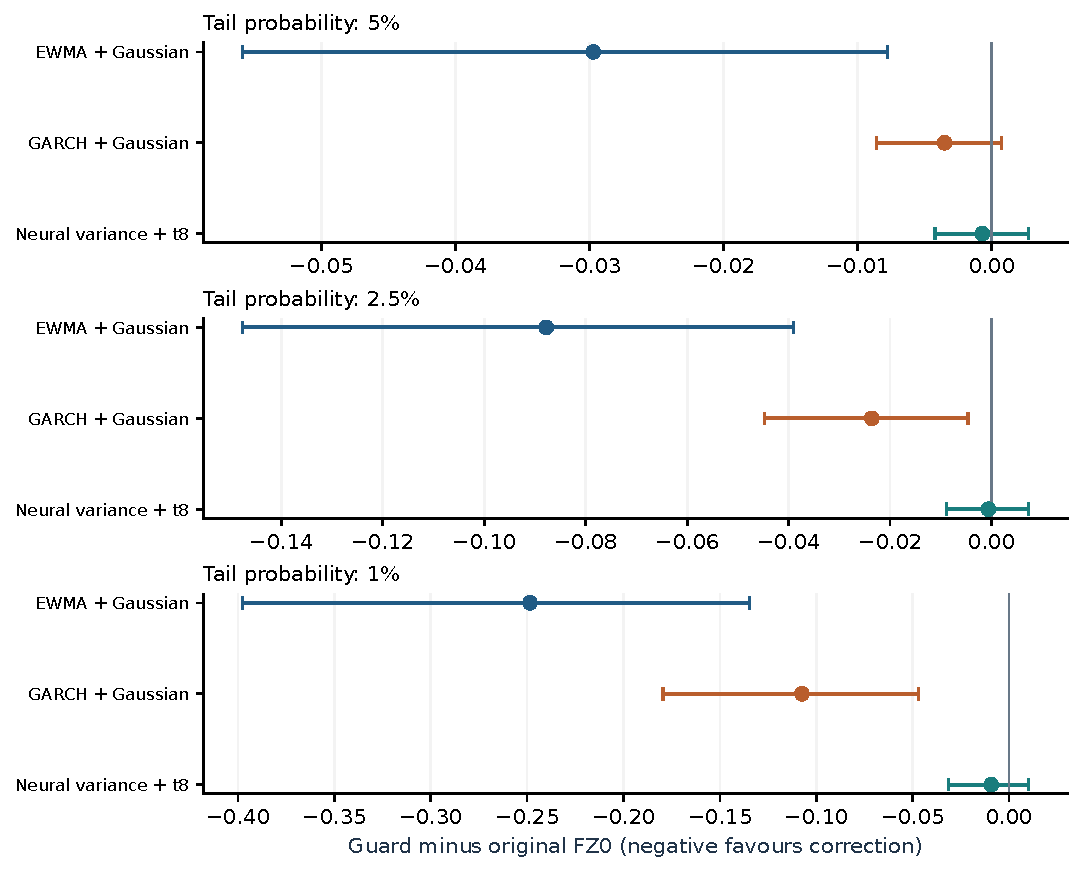
\includegraphics[width=0.94\textwidth]{figures/tail_effect_by_starting_model.pdf}
\caption[Historical tail correction by original forecast]{Historical later-block score changes for the development-selected, 1,000-observation guard. Negative values favour correction. The error bars are the archived individual 95\% calendar-block intervals; the separate Holm adjustment is reported in Table~\ref{tab:tail-m1}. Horizontal scales differ across panels to keep small effects visible. The neural row uses the retained variance path with $t_8$ tails. Specialist rows retain the original optimiser acceptance policy.}
\label{fig:tail-starting-model}
\end{figure}

Gaussian tails leave substantial error to repair here. A more flexible distribution may already capture much of the tail shape, so the gains do not support a universal improvement claim. We next evaluate correction of the archived neural variance forecast with Student tails.

\section{Neural forecasts: coverage improves, score gains remain uncertain}

For the retained neural variance path with Student tails, the table uses corrected-minus-original FZ0: negative differences favour correction. Its marginal intervals concern individual comparisons.

\begin{table}[htbp]
\centering
\caption[Neural-tail joint-score comparisons]{Neural variance with Student-$t(8)$ tails: fixed guard minus original FZ0. Intervals are marginal calendar-block bootstrap intervals, with no multiplicity adjustment.}
\label{tab:tail-neural}
\small
\begin{tabular}{lrrrr}
\toprule
Panel & $\alpha$ & Difference & 95\% interval & Raw $p$\\
\midrule
Development & .050 & +.00019 & $[-.00462,\phantom{-}.00402]$ & .878\\
 & .025 & +.00092 & $[-.00606,\phantom{-}.00629]$ & .716\\
 & .010 & +.00323 & $[-.00170,\phantom{-}.00711]$ & .170\\
\midrule
Later & .050 & -.00071 & $[-.00424,\phantom{-}.00271]$ & .665\\
 & .025 & -.00064 & $[-.00889,\phantom{-}.00722]$ & .872\\
 & .010 & -.00928 & $[-.03137,\phantom{-}.00991]$ & .358\\
\bottomrule
\end{tabular}
\end{table}

Every interval for corrected-minus-original neural FZ0 crosses zero (Table~\ref{tab:tail-neural}). Development means slightly favour the original, and later means favour the guard. Even the later 1\% interval permits benefit or deterioration. The joint-score evidence consequently leaves neural improvement unresolved.

The unconditional breach diagnostic improves more clearly. At the later 1\% level, the number of markets inside the nominal binomial frequency band rises from twelve to 27 of 28, while mean breach frequency falls from about 1.5\% to 1.3\%. Using actual market sample sizes retains that count. These frequencies do not establish conditional coverage, accurate ES or joint-score improvement.

\begin{figure}[htbp]
\centering
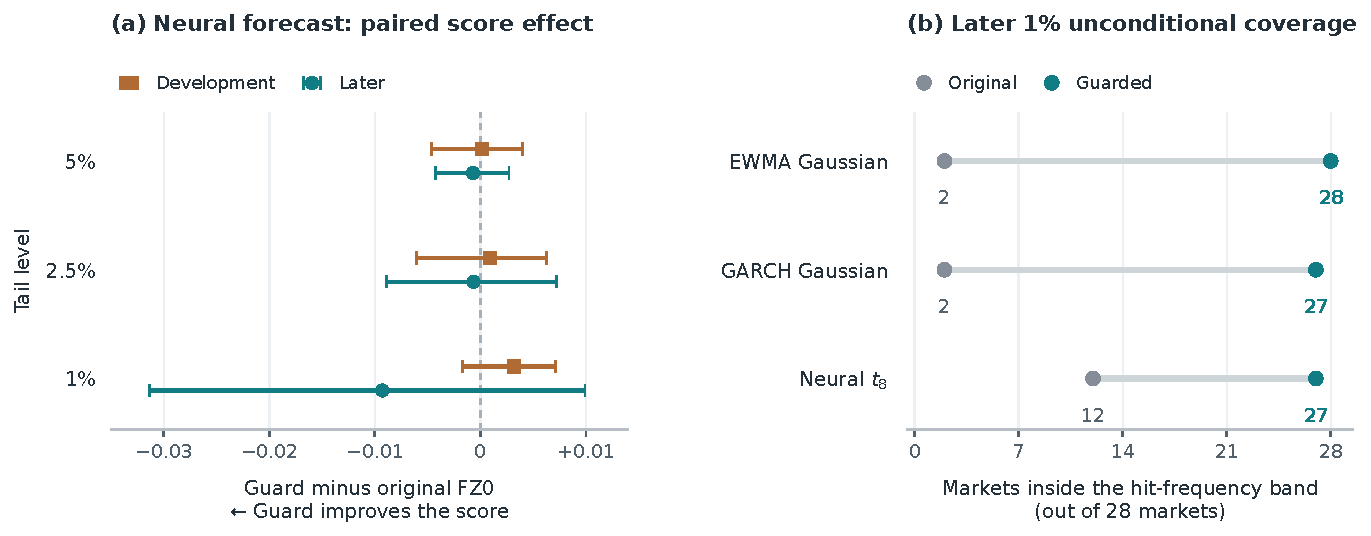
\includegraphics[width=\textwidth]{figures/tail_diagnostics_new.pdf}
\caption[Joint-score uncertainty and unconditional coverage]{Two distinct diagnostics of fixed tail recalibration. (a) Neural variance with Student-$t(8)$ tails: guard-minus-original FZ0 differences and marginal 95\% calendar-block bootstrap intervals. Every interval includes zero. Development uses the full-history guard (\code{guard\_ftl}); the later panel uses the development-selected 1,000-observation guard (\code{guard\_win1000}). (b) Later $1\%$ numbers of markets inside the historical central binomial hit-frequency band before and after that selected guard. The band uses the panel sample-size convention $n=1{,}788$; these are unconditional frequency screens, not conditional coverage tests.}
\label{fig:tail-diagnostics-new}
\end{figure}

Figure~\ref{fig:tail-diagnostics-new} shows this distinction between improved breach counts and uncertain joint scores. Equal counts can also conceal crisis clustering \citep{kupiec1995techniques,christoffersen1998evaluating}. Mean ES residuals decline descriptively, but their archived summaries have no intervals (Appendix~\ref{app:results}). These summaries describe observed severity errors without resolving joint-score uncertainty.

We also assess practical loss tolerances for specialist models. In the convergence-checked later panel, the GAS guard at 1\% exceeds its tolerance. One supplementary unguarded GAS decision at 2.5\% changes from pass to fail, while its guarded counterpart passes. Appendix~\ref{sec:optimizer-sensitivity} separates these changes from the historical tables. Passing a point tolerance is not statistical proof of no harm, and failing it is not statistical proof of harm.

\section{Comparison with filtered historical simulation}

Chapter~\ref{ch:recalibration} shows that fixed-shape ratio correction is FHS expressed through absolute VaR. A claim beyond Gaussian repair therefore requires comparison with FHS. Here FHS refreshes its residual pair at expanding GARCH refits, whereas ratio correction updates sequential residuals daily and the guard may retain the original Gaussian pair. Both updating and selection differ, preventing attribution to selection alone.

\begin{figure}[!htbp]
\centering
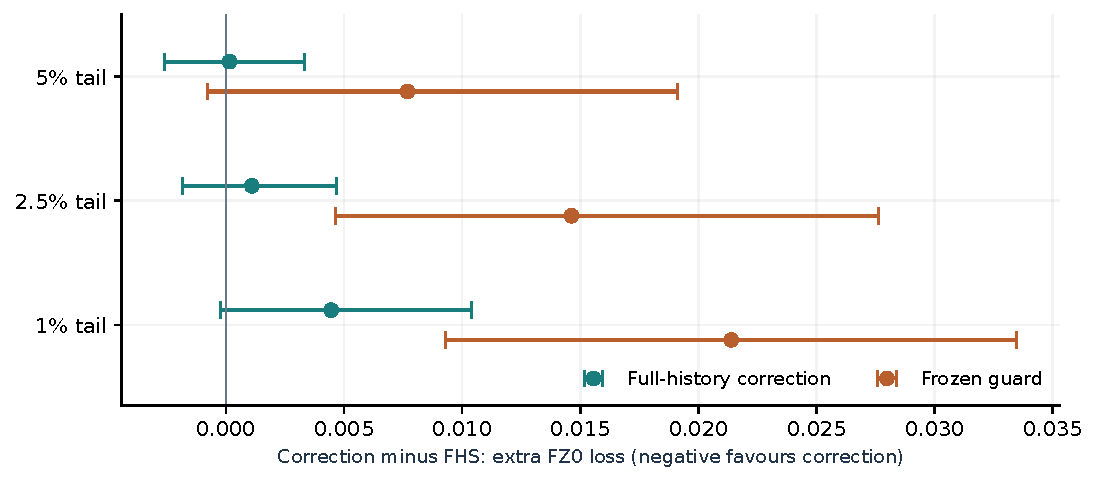
\includegraphics[width=\textwidth]{tail_fhs_comparison.pdf}
\caption[Historical residual correction and guard against FHS]{Historical later 28-market panel: Gaussian-GARCH full-history ratio correction and the frozen guard, each minus GARCH FHS. Positive values mean higher loss than FHS. Bars are archived marginal 95\% calendar-block intervals for these supplementary, post-hoc matched-date comparisons. All GARCH procedures retain the original optimiser acceptance policy. The correction and guard use different residual-history rules, so the comparison does not isolate selection alone.}
\label{fig:tail-fhs}
\end{figure}

On matched dates, full-history correction has similar means to FHS, but all six marginal intervals cross zero. The frozen later guard has higher FZ0 at 2.5\% and 1\%, by about 0.015 and 0.021. These post-hoc comparisons use unadjusted tests, with exact results retained in Appendix~\ref{app:results}. Convergence-checked refitting preserves both findings (Table~\ref{tab:optimizer-fhs-sensitivity}). We establish neither full-history equivalence nor general superiority over FHS.

A guard can avoid an unsuitable correction or discard a useful one (Figure~\ref{fig:tail-fhs}). It must therefore be evaluated as a forecasting procedure, and these results do not generally favour the fixed guard.

\section{Exploratory adaptation and the resulting conclusion}

The exploratory selector chooses among the original and several residual histories. It passes 39 of 57 simulation checks and more later market checks than the fixed guard. However, its design followed inspection of that period; causal updating cannot remove this research exposure. Convergence-checked replay changes no decisions, and Appendix~\ref{app:results} preserves counts and candidates.

Correction helps most clearly with Gaussian tails. Neural joint-score gains remain inconclusive, and the fixed guard sometimes loses to FHS. The simulations show how starting tail error, estimation cost and residual history affect these outcomes within the tested settings; they supply no universal guarantee.

Correction needs to add value over both the original forecast and an established residual alternative. Chapter~\ref{ch:discussion} relates this qualified answer to the prior and compact-recovery findings.